\documentclass[11pt]{article}
\usepackage{amsfonts}
\usepackage{amsmath}
\usepackage{hyperref}
\usepackage{esvect} 
\usepackage[boldfont]{xeCJK}

\begin{document}

\title{Mathematical Knowledge\\ for Dynamical Modeling of Quadrotors}
\author{Shuo Yang}
\maketitle
This tutorial aims to provide engineers and researchers who are interested in understanding basic mathematical knowledge used in modeling and control of multirotor aerial robots. I introduce rotation representation, angular velocity, inertia, Euler Angle and Euler Equation in the tutorial.

Engineers and scientists who study multirotor aerial robots mainly have EE, MECH, CS background. Most of them only studied basic math and physics course, without systematical training on classical mechanics and algebra. However, to deeply understand necessary engineering practice for multirotor aerial robot, people have to gain better understanding of more knowledge beyond simple linear algebra.

Nevertheless, following traditional math and physics courses for engineering students is time consuming. I think it is easier for students to study math and physics through studying one of the core topics of aerial robotics, namely dynamic modeling. Because dynamic modeling has a clear workflow to apply math and physic. Each math or physic concept, once been presented in the tutorial, will be immediately applied to solve real engineering problems or understand real world engineering phenomenon.

This tutorial tries to use standardized notations and detailed derivations to introduce math and physics concepts. I try not to neglect intermediate steps when I derive equations.

\section{Basic Notations \& Coordinate Frames}
This section states some basic notations and coordinate frame conventions used in aerial vehicle control. The whole tutorial will only use these notations.
\subsection{Basic Notations}
$a$, alphabet letters represent scalar. They can also be names of certain concepts, for example $x$-axis of a coordinate frame.

$\vv{v}$, alphabet letters with overhead arrow stand for vector. Many teaching materials use bold letters, such as $bf{v}$ to represent vector, which confuses vector with matrix and scalar at the same time. In this tutorial I never drop overhead arrow of vectors to keep notifying readers about the meaning of a quantity.

$\dot{a}$, the derivative of a scalar function $a(t)$. We drop$(t)$ to simplify notation.

$\dot{\vv{v}}$ or $\frac{d\vv{v}}{dt}$, means the derivative of a vector function. We implicitly assume every element of vector $\vv{v}$ is a scalar function of time $t$.

$\bf{A}$, is a matrix. 

$\bf{I}_{3x3}$, sometimes subscript will be added to denote the size of the matrix. A common example is to indicate the size of identity matrix $\bf{I}$. If the matrix has 3 columns and 3 rows, than the matrix is denoted as $\bf{I}_{3x3}$.

$\bf{A}^{-1}$, is the inverse of a matrix.

$\bf{A}^T$, is the transpose of a matrix.

$\bar{\bf{q}}$ represents a quaternion.

${\bf R}_{ab}$ is a rotation matrix. $a$和$b$ are two coordinate frame with \textbf{coincide origin}. The rotation matrix rotates vector represented in frame $b$ to representation in frame $a$.

$\bar{\bf{q}}_{ab}$ stands for a rotation quaternion. The meaning of its subscript is same as the rotation matrix.

$\lfloor \vv{\omega} \ \times \rfloor$ denotes an operation that transforms vector $\vv{\omega}$ to skew symmetric matrix $\lfloor \vv{\omega} \ \times \rfloor$.

Other undefined symbols will be introduced in the tutorial text.
\subsection{Coordinate Frames}
Aerospace and aeronautical engineers have developed a standard convention to describe the position of an aerial vehicle relative to the surface of the earth. This convention includes two coordinate frames, namely ground frame and body frame.
\subsubsection{Ground Frame}
An aerial vehicle initializes at a spot on the ground. After the aerial vehicle starts moving, many sensors on the vehicle still take this initial spot as a reference point. To describe the relative position and 

\section{Understand Quadrotor by Simulation}

This tutorial introduces rotation matrix, angular velocity, Euler equation and related mathematical knowledge used in multirotor aerial robotics. Gyroscope and multirotor are two main topics that link engineering and mathematics.  


In \url{https://github.com/paulyang1990/toy_code/tree/master/toy_ros_space/src/sim_drone} I implemented a simple quadrotor simulator. File rigidBody.cpp demonstrates how to realize discrete Euler equation simulation.

\begin{center}
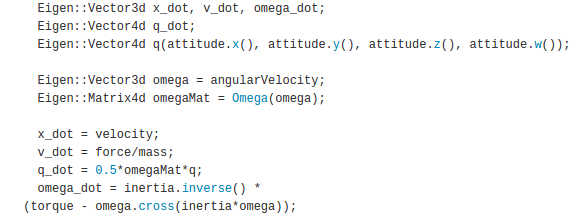
\includegraphics[width=0.9\textwidth]{images/code.png}
\end{center}

Readers can use rigidBody.cpp and related assist code to understand Euler equation by themselves.

\bibliographystyle{plain}
\bibliography{tutorial}
\end{document}